\section{Experimental Evaluation}

\def\arraystretch{1.1}

% Please add the following required packages to your document preamble:
% \usepackage{multirow}
% \usepackage{graphicx}
\begin{table*}[ht]
\centering
\resizebox{\textwidth}{!}{%
\begin{tabular}{ll|l|llll|llll|llll}
                                                                                                         &               & \multicolumn{1}{c|}{\multirow{2}{*}{\ssb}} & \multicolumn{4}{c|}{\ssp}                                      & \multicolumn{4}{c|}{\ssc}                                       & \multicolumn{4}{c}{\ssm}                                      \\
                                                                                                         	&	 type          	&	 \multicolumn{1}{c|}{}                      	&	 \pss            	&	 \psa          	&	 \psr          	&	 \psd         	&	 \pss            	&	 \psa          	&	 \psr          	&	 \psd          	&	 \pss          	&	 \psa          	&	\psr	&	 \psd          	\\	\hline
\multicolumn{1}{l|}{\multirow{4}{*}{\begin{tabular}[c]{@{}l@{}}Used\\ vertices\end{tabular}}}            	&	 \emph{empty}  	&	1	&	 \textbf{0.14}   	&	0.23	&	0.21	&	0.23	&	 \textbf{0.15}   	&	0.24	&	0.22	&	0.23	&	0.19	&	0.24	&	0.23	&	0.24	\\
\multicolumn{1}{l|}{}                                                                                    	&	 \emph{maze}   	&	1	&	 \textbf{0.18}   	&	0.2	&	 \textbf{0.18} 	&	0.19	&	 \textbf{0.20}   	&	0.22	&	0.21	&	0.21	&	0.22	&	0.22	&	0.22	&	0.22	\\
\multicolumn{1}{l|}{}                                                                                    	&	 \emph{random} 	&	1	&	 \textbf{0.19}   	&	0.27	&	0.24	&	0.25	&	 \textbf{0.22}   	&	0.3	&	0.28	&	0.29	&	0.25	&	0.31	&	0.3	&	0.31	\\
\multicolumn{1}{l|}{}                                                                                    	&	 \emph{room}   	&	1	&	 \textbf{0.21}   	&	0.24	&	0.22	&	0.22	&	 \textbf{0.23}   	&	0.27	&	0.25	&	0.25	&	0.24	&	0.29	&	0.27	&	0.28	\\	\hline
\multicolumn{1}{l|}{\multirow{4}{*}{\begin{tabular}[c]{@{}l@{}}Solved\\ instances\end{tabular}}}         	&	 \emph{empty}  	&	0.78	&	 \textbf{0.99}   	&	0.81	&	0.84	&	0.82	&	 \textbf{1.00}   	&	0.81	&	0.84	&	0.82	&	0.87	&	0.81	&	0.82	&	0.8	\\
\multicolumn{1}{l|}{}                                                                                    	&	 \emph{maze}   	&	0.85	&	0.87	&	 \textbf{0.88} 	&	0.87	&	0.87	&	 \textbf{0.98}   	&	0.97	&	0.97	&	 \textbf{0.98} 	&	0.94	&	0.94	&	0.94	&	0.94	\\
\multicolumn{1}{l|}{}                                                                                    	&	 \emph{random} 	&	0.79	&	 \textbf{0.91}   	&	0.82	&	0.84	&	0.84	&	 \textbf{1.00}   	&	0.89	&	0.92	&	0.91	&	0.93	&	0.87	&	0.89	&	0.88	\\
\multicolumn{1}{l|}{}                                                                                    	&	 \emph{room}   	&	0.8	&	 \textbf{0.83}   	&	0.81	&	0.82	&	0.82	&	 \textbf{0.97}   	&	0.92	&	0.95	&	0.94	&	0.89	&	0.89	&	0.89	&	0.89	\\	\hline
\multicolumn{1}{l|}{\multirow{5}{*}{$\sum$ IPC}}                                                         	&	 \emph{empty}  	&	874.6	&	 \textbf{1930.5} 	&	1312.8	&	1081.7	&	1086.3	&	 \textbf{2395.2} 	&	1276.5	&	1406.7	&	1324.4	&	1517.9	&	1275.8	&	1312.5	&	1279.2	\\
\multicolumn{1}{l|}{}                                                                                    	&	 \emph{maze}   	&	890.1	&	 \textbf{1153.2} 	&	1123.6	&	1128.3	&	1143.3	&	 \textbf{1775.5} 	&	1633.8	&	1752.8	&	1754	&	1475.7	&	1452.6	&	1470.5	&	1466.1	\\
\multicolumn{1}{l|}{}                                                                                    	&	 \emph{random} 	&	886	&	 \textbf{1668.0} 	&	1110.2	&	1049.9	&	1102.3	&	 \textbf{2275.5} 	&	1422.4	&	1594.6	&	1551.5	&	1560.7	&	1300.3	&	1374.2	&	1324.4	\\
\multicolumn{1}{l|}{}                                                                                    	&	 \emph{room}   	&	877.3	&	 \textbf{1386.4} 	&	1007.5	&	1191.6	&	1179.5	&	 \textbf{2078.3} 	&	1594.5	&	1850.6	&	1828.7	&	1474	&	1382.6	&	1461.9	&	1442	\\	\cline{2-15}
\multicolumn{1}{l|}{}                                                                                    	&	 total         	&	3527.9	&	 \textbf{6138.1} 	&	4554.1	&	4451.6	&	4511.4	&	 \textbf{8524.5} 	&	5927.2	&	6604.6	&	6458.6	&	6028.4	&	5411.3	&	5619.2	&	5511.6	\\	\hline
\multicolumn{1}{l|}{\multirow{4}{*}{\begin{tabular}[c]{@{}l@{}}Solved\\ optimally\end{tabular}}}         	&	 \emph{empty}  	&	 -                                          	&	 -               	&	 -             	&	 -             	&	 -            	&	0.93	&	 \textbf{1.00} 	&	 \textbf{1.00} 	&	 \textbf{1.00} 	&	 \textbf{1.00} 	&	 \textbf{1.00} 	&	\textbf{1.00}	&	 \textbf{1.00} 	\\
\multicolumn{1}{l|}{}                                                                                    	&	 \emph{maze}   	&	 -                                          	&	 -               	&	 -             	&	 -             	&	 -            	&	0.91	&	 \textbf{0.94} 	&	0.92	&	0.92	&	0.92	&	0.93	&	0.93	&	0.93	\\
\multicolumn{1}{l|}{}                                                                                    	&	 \emph{random} 	&	 -                                          	&	 -               	&	 -             	&	 -             	&	 -            	&	0.89	&	 \textbf{0.97} 	&	0.95	&	0.96	&	0.86	&	0.91	&	0.91	&	0.91	\\
\multicolumn{1}{l|}{}                                                                                    	&	 \emph{room}   	&	 -                                          	&	 -               	&	 -             	&	 -             	&	 -            	&	0.86	&	 \textbf{0.93} 	&	0.91	&	0.92	&	0.76	&	0.86	&	0.85	&	0.85	\\	\hline
\multicolumn{1}{l|}{\multirow{4}{*}{Conflicts}}                                                          	&	 \emph{empty}  	&	133	&	 \textbf{97}     	&	148	&	131	&	136	&	 \textbf{111}    	&	147	&	141	&	142	&	139	&	148	&	146	&	148	\\
\multicolumn{1}{l|}{}                                                                                    	&	 \emph{maze}   	&	2457	&	 \textbf{1239}   	&	1804	&	1274	&	1265	&	3101	&	 \textbf{2969} 	&	3120	&	3143	&	3361	&	3482	&	3443	&	3354	\\
\multicolumn{1}{l|}{}                                                                                    	&	 \emph{random} 	&	206	&	193	&	195	&	174	&	 \textbf{173} 	&	 \textbf{218}    	&	235	&	234	&	227	&	448	&	458	&	460	&	459	\\
\multicolumn{1}{l|}{}                                                                                    	&	 \emph{room}   	&	1007	&	402	&	313	&	270	&	 \textbf{289} 	&	1642	&	1414	&	1513	&	1423	&	1525	&	 \textbf{1400} 	&	1527	&	1545	\\	\hline
\multicolumn{1}{l|}{\multirow{4}{*}{\begin{tabular}[c]{@{}l@{}}Constraints\\ {[millions]}\end{tabular}}} 	&	 \emph{empty}  	&	 \textbf{4.7}                               	&	7.3	&	5.1	&	5.9	&	5.2	&	7.4	&	5.1	&	6	&	5.2	&	6	&	 \textbf{5.0}  	&	5.2	&	 \textbf{5.0}  	\\
\multicolumn{1}{l|}{}                                                                                    	&	 \emph{maze}   	&	 \textbf{6.0}                               	&	6.1	&	6.4	&	6	&	6.2	&	 \textbf{6.4}    	&	6.8	&	6.5	&	6.6	&	6.8	&	6.8	&	6.8	&	6.8	\\
\multicolumn{1}{l|}{}                                                                                    	&	 \emph{random} 	&	 \textbf{5.4}                               	&	5.9	&	6	&	6	&	6	&	6	&	6.1	&	6.1	&	6.1	&	6.1	&	 \textbf{5.8}  	&	6	&	 \textbf{5.8}  	\\
\multicolumn{1}{l|}{}                                                                                    	&	 \emph{room}   	&	 \textbf{4.8}                               	&	5.4	&	5.6	&	5.4	&	5.4	&	 \textbf{5.7}    	&	5.9	&	5.8	&	 \textbf{5.7}  	&	 \textbf{5.7}  	&	5.9	&	5.9	&	5.9
\end{tabular}%
}
\caption{Ratio of used vertices, ratio of solved instances,  sum of IPC score, ratio of instances solved optimally, average number of conflicts, and average number of constraints. The results are split by the map type. Strategies are \emph{baseline} (\ssb{}), \emph{prune-and-cut} (\ssp{}), \emph{makespan-add} (\ssm{}), and \emph{combined} (\ssc{}). Approaches to choosing shortest paths are \emph{single-path} (\pss), \emph{all-paths} (\psa), \emph{random-paths} (\psr), and \emph{distant-paths} (\psd).}
\label{tab:results}
\end{table*}


To test and compare the proposed strategies in combination with approaches to creating the restricted graph, we set up experiments. The full implementation and results are available at \url{https://github.com/potassco/mapf-subgraph-system}. For the ASP-based solver, we used the grounding-and-solving system \emph{clingo}~\cite{PotasscoUserGuide19,karoscwa20a} version~\(5.5.2\). We ran the experiments on an Intel Xeon E5-2650v4 under Debian GNU/Linux~9, with each instance limited to 300s processing time and 28 GB of memory.


% \subsection{Instances}
%
The instances used in our experiments are based on commonly used benchmark instances available online~\cite{stern2019mapfVarians}. We chose different sizes of maps -- \emph{small} (32 by 32), \emph{medium} (64 by 64), and \emph{large} (128 by 128) and different structures of the impassable obstacles in the map with the following types -- \emph{empty}, \emph{maze}, \emph{random}, and \emph{room}. % (see Figure~\ref{fig:maps} for reference). Unfortunately, some of the combinations of size and type were not available in the benchmark set, therefore, we had to create our own following the structure of the existing maps.

%\begin{figure}[ht]
%\centering
%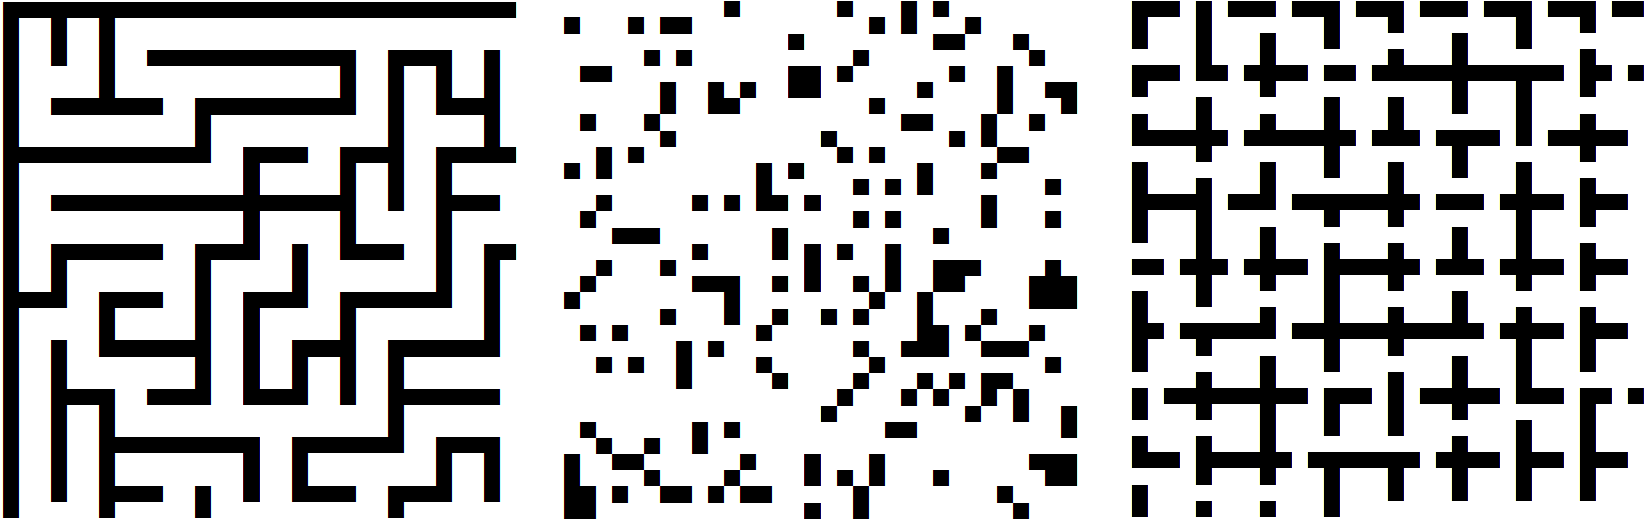
\includegraphics[width=0.75\columnwidth]{img/maps_32.png}
%\caption{Types of maps used in the experimental evaluation. From left to right: \emph{maze}, \emph{random}, and \emph{room}.}
%\label{fig:maps}
%\end{figure}

For the placement of the agents (called \emph{scenarios}), we used the available scenarios. % from the benchmark sets or, if not present, created our own. For each map, we used 5 different scenarios.
Furthermore, we created new scenarios for each map such that the distance from start to goal of each agent is similar and the paths of the agents need to cross more often. We did this because the makespan optimal solution for the random scenarios rarely differs from the lower bound. %This is caused by one of the agents having a much longer path than the others leaving them with enough time to solve any conflicts.
The behavior of the strategies may be gravely affected by many conflicts and the need to increase the makespan.% We are also using 5 different scenarios with this setting.

The intended way to use the benchmark set is to create an instance of MAPF from a map and a number of agents from a scenario. If the instance is solved in the given time limit, an additional agent from the same scenario is added and thus a new MAPF instance is produced. Once the instance cannot be solved in the time limit, it is reasoned that increasing further the number of agents cannot make the instance solvable. We are aware that using a reduction-based solver, this may not always hold. Also, some of the strategies may benefit from additional agents which change the restricted graph. However, these cases are extremely rare and therefore, we decided to use the benchmark as intended.


%\subsection{Results}
%
Table~\ref{tab:results} shows the results for all of the strategies and approaches to creating the restricted graph. Note that the \emph{baseline} strategy \ssb{} considers the whole map, therefore we do not use any of the four approaches. The strategies \ssb{} and \ssp{} are optimal, therefore, we will consider them separately opposed to the suboptimal strategies \ssc{} and \ssm{}. The best result for both optimal and suboptimal strategies on each line is highlighted. We present the results divided by the type of the map regardless of the size. This representation shows nicely the difference between the approaches to creating the restricted graph. For more detailed results, we include much more detailed tables in the supplementary materials.

First, we examine the average number of vertices used by each approach. In the table, the number indicates the ratio of used vertices to the total number of vertices. Since \ssb{} always uses the whole map, the ratio is $1$. We can see that \pss{} uses the least number of vertices in all cases, on the other hand, \psa{} uses the most and \psd{} and \psr{} use about the same. This result is not surprising since it is based on the number of paths used by each approach. However, we can also see that the difference is much bigger on opened maps (such as \emph{empty}) and much smaller on very restrictive maps (such as \emph{maze}), meaning that in the latter case there are not many different shortest paths for the agents to choose from. There is also a clear order in terms of the strategies with \ssp{} using the least, \ssc{} using more, and \ssm{} using even more vertices on average.

Examining the number of solved instances (ratio of solved to all instances -- 2544 for \emph{empty}, 1956 for \emph{maze}, 2418 for \emph{random}, 2357 for \emph{room}), we see that the most successful combination is \ssp{} + \pss{} for the optimal setting and \ssc{} + \pss{} for the suboptimal. Again the difference across the approaches to choosing the shortest paths is least prominent on \emph{maze} maps, however, on the other types, the order is clear. The \pss{} is the most successful, \psd{} and \psr{} performing about the same, while \psa{} performs the worst. The \emph{baseline} \ssb{} performs worse than any other used combination.
Similar results can be seen when exploring the IPC score~\footnote{introduced at International Planning Competition, hence the name.} (Computed as 0 if the solver did not finish in time, otherwise as $\frac{\textit{min. time}}{\textit{solver time}},$ where \textit{min. time} is the time it took the fastest solver and \textit{solver time} is the time it took the solver in question. The score ranges from 0 to 1, where the bigger the number the better. The scores of all instances are summed) For the \ssp{} strategy the \psa{} approach performs better than \psd{} and \psr{}, meaning that while it did not solve more instances, the instances it managed to solve were solved faster. For the other strategies, the order remains the same as with the number of solved instances. It is unsurprising that the suboptimal strategies achieved a better score that the optimal \ssp{}.

We argue that these results stem from the number of used vertices. By exploring the ASP solver, we see that for all strategies and all additional shortest path approaches, the number of conflicts stays mostly within the same order of magnitude as for \pss{}. Hence, ASP search difficulty remains unchanged.
However, compared to \pss{}, the other approaches add more vertices to the restricted graph to consider and, in consequence, this increases the grounding time of \emph{clingo} which, in turn, leads to more timeouts.
%esp. for instances that finished close to 300s, for \pss{}.

The new shortest path approaches reduce the size of the internal problem specification in terms of the number of constraints.
We conjecture that since the new approaches generally select multiple (and more likely exclusively usable by one agent) vertices for the restricted graph, the amount of constraints encoding possible agent collisions is reduced. However, as mentioned above, this has no significant impact on the search complexity.

We also explore the quality of the solutions produced by the suboptimal strategies. The ratio of instances solved optimally is again shown in Table~\ref{tab:results}. Strategy \ssc{} is more often optimal compared to \ssm{}. This time, we can see the benefit of adding extra vertices to the restricted graph. The most often optimal approach is \psa{} closely followed by \psr{} and \psd{}, while \pss{} achieved the worst results. The difference is again less prominent on \emph{maze} maps.

%%% Local Variables:
%%% mode: latex
%%% TeX-master: "main"
%%% End:
